\documentclass[a4paper,12pt]{article}
\usepackage[margin=1in]{geometry}

\usepackage[T2A]{fontenc}			% кодировка
\usepackage[utf8]{inputenc}			% кодировка исходного текста
\usepackage[english,russian]{babel}	% локализация и переносы
\usepackage{graphicx}                % Математика
\usepackage{amsmath,amsfonts,amssymb,amsthm,mathtools} 
\usepackage{mathtext}
\usepackage[T2A]{fontenc}
\usepackage[utf8]{inputenc}

\usepackage{wasysym}
\renewcommand{\theenumii}{\arabic{enumii}}

%Заговолок
\author{Бичина Марина 
группа Б04-005 1 курса ФЭФМ}
\title{}
\date{}


\begin{document} % начало документа

\begin{center}
\begin{Large}
{Бичина Марина Б04-005, Лабораторная работа №.5.8.1 <<Определение постоянных Стефана-Больцмана и Планка из анализа теплового излучения накаленного тела>> }
\end{Large}
\end{center}
\paragraph{Цель работы:} 
\begin{enumerate}
\itemsep0em
\item Измерить температуры оптическим пирометром с исчезающей нитью
\item Измерить температуру с помощью термопары
\item Исследовать излучение накаленных тел с различной испускательной способностью
\item Определить постоянные Планка  Стефана-Больцмана
\end{enumerate}
\paragraph{Оборудование:}
\begin{enumerate}
\itemsep0em
\item оптический пирометр
\item модель АЧТ
\item образцы колец
\item вольфрамовая лампа
\item неоновая лампа
\item блок питания
\item цифровые вольтметры
\end{enumerate}
\paragraph{Теоретическая справка:}
\paragraph{}
В оптической пирометрии различают три температуры, функционально связанные с истинной термодинамической температурой и излучательной способностью тела: \textbf{радиационную $T_{\text{рад}}$, цветовую $T_{\text{цв}}$ и яркостную $T_{\text{ярк}}$}. В работе измеряется яркостная температура. \\
\textit{Яркостная температура} - это температура абсолютно чёрного тела, при которой его спектральная испускательная способность равна спектральной испускательной способности исследуемого тела при той же длине волны.\\
Измерение яркостной температуры раскалённого тела производится при помощи оптического пирометра с исчезающей нитью, основанного на визуальном сравнении яркости раскалённой нити с яркостью изображения исследуемого тела. \\
Яркостная температура тела всегда ниже его термодинамической температуры. Это связано с тем, что любое нечёрное тело излучает меньше, чем АЧТ при той же температуре. Зависимость между яркостной и термодинамической температурами вольфрама приведена на рис. 1

\begin{figure}[h]
    \centering
    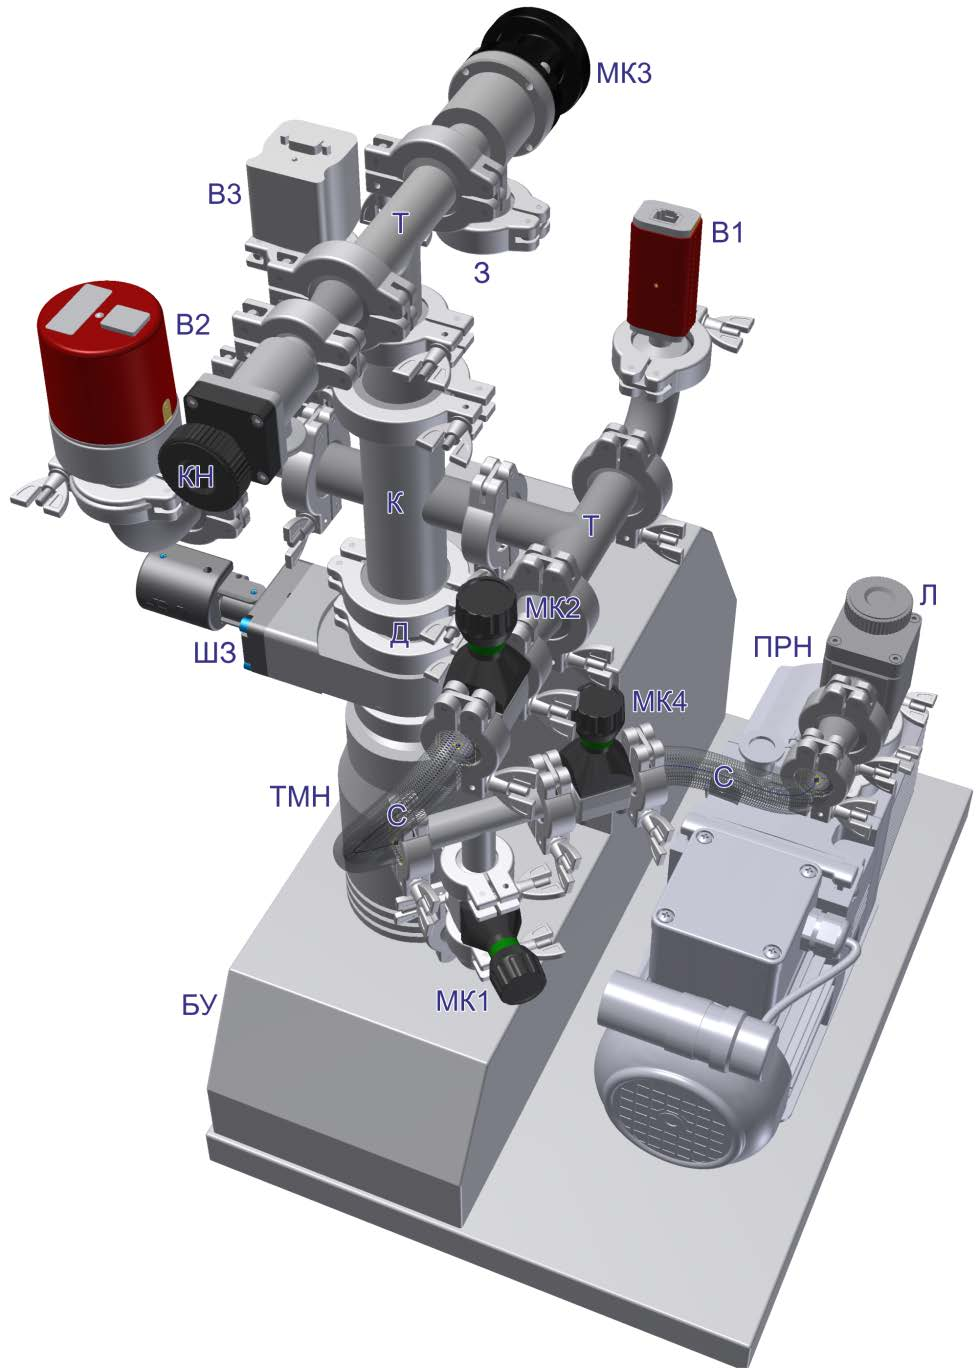
\includegraphics[width=10cm]{fig2.PNG}
    \caption{График зависимости $T = f(T_{\text{ярк}})$ для вольфрама}
    \label{fig:vac}
\end{figure}

По результатам измерений мощности излучения вольфрамовой нити можно судить о справедливости закона Стефана-Больцмана. Если бы нить излучала как АЧТ, то баланс потребляемой и излучаемой энергии определялся бы соотношением 
\begin{equation}
    W = \sigma S (T^4 - T_0^4),
\end{equation}
где $W$ - потребляемая нитью электрическая мощность, $S$ - площадь излучающей поверхности нити, $T$ - температура нити, $T_0$ - температура окружающей среды. Однако вольфрамовая нить излучает как серое телo, и излучение её ослаблено по сравнению с АЧТ в $\varepsilon_T$ раз для любой волны при данной температуре тела Т. Тогда предположив, что нить излучает как серое тело и с учётом того, что $T_0 \ll T$, выражение (1) можно переписать в виде
\begin{equation}
    W = \varepsilon_T S \sigma T^4
\end{equation}
В справедливости закона Стефана-Больцмана можно убедиться, построив график зависимости $W(T)$ в логарифмическом масштабе и по углу наклона определить показатель степени $n$ исследуемой температурной зависимости. В пределах погрешности показатель степени должен быть близок к четырём. \\
Также из формулы (2) можно определить постоянную Стефана-Больцмана.

\paragraph{Описание установки:}
\begin{figure}[h!]
\centering
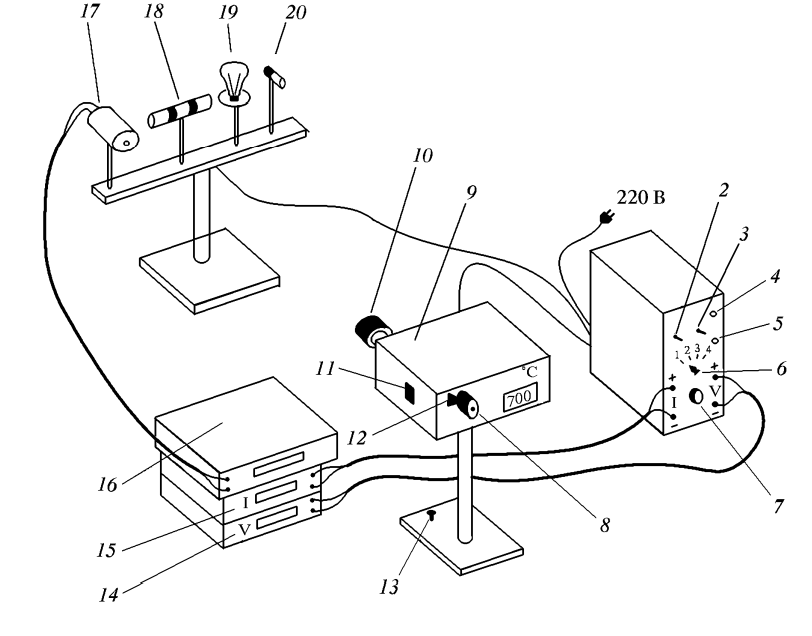
\includegraphics[scale=0.5]{setup.png}
\caption{Cхема экспериментальной установки} 
\end{figure}
\paragraph{}
Основные элементы установки:\\
1 -- блок питания\\
9 -- пирометр в двух диапазонах: $700-1200 ^oC$ и $1200-2000^oC$\\
14 -- вольтметр (напряжение на лампе накаливания)\\
15 -- амперметр (ток через образцы)\\
16 -- вольтметр (цепь термопары)\\
17 -- модель АЧТ\\
18 -- трубка с кольцами из материалов с разной излучательной способностью\\
19 -- лампа накаливания\\
20 -- неоновая лампочка
\newpage
\paragraph{Ход работы:}
\begin{enumerate}
\itemsep0em
\item \textbf{Изучение работы оптического пирометра}
\begin{enumerate}
\itemsep0em
\item Прогреем модель АЧТ. Настроим пирометр на необходимый диапазон температур.
\item Снимем показания пирометра: для этого, глядя в оптическую трубу, будем изменять ток, пропускаемый через нить пирометра, до тех пор, пока нить не исчезнет на фоне раскаленной поверхности АЧТ.
\item Измерим температуру АЧТ при помощи термопары
\item Полученные данные сведем в таблицу $\ref{thermopiro}$
\item Видим, что для данных измерений погрешность составляет менее 5$\%$. Следовательно, для АЧТ корректно определять температуру таким способом.
\end{enumerate}
\begin{table}[h!]
\centering
\begin{tabular}{|l|l|l|l|}
\hline
температура, снятая с помощью пирометра, $^oC$ & 939  & 948  & 956  \\ \hline
напряжение, на термопаре, мВ                   & 38.6 & 38.7 & 39.0 \\ \hline
температура, снятая с помощью термопары, $^oC$ & 941  & 944  & 951  \\ \hline
\end{tabular}
\caption{Температура АЧТ}
\label{thermopiro}
\end{table}
\item \textbf{Измерение яркостной температуры тел}\\
Покажем, что разные тела, нагретые до одинаковой термодинамической температуры,имеют различную яркостную температуру
\begin{enumerate}
\item Прогреем керамическую трубку с кольцами.
\item Пронаблюдаем за образцами: Видим, что один образец изменил цвет на ярко-красный, другой остался практически таким же темным.
\item Сделаем вывод о том, что яркостная и термодинамическая температура могут не совпадать. Это может быть связано с тем, что обе величины связаны через спектральный коэффициент поглощения, который различен у разных материалов.
\end{enumerate}
\item \textbf{Проверка закона Стефана-Больцмана}
\begin{enumerate}
\item Рассмотрим диапазон, в котором мы можем снимать показания: для нас это с 1.33 мА (при меньшем токе нить накала не горит) до 8 мА (максимальный ток). В данном диапазоне снимем 20 точек.
\item Полученные данные занесем в таблицу $\ref{lampa}$
\item Удостоверимся в справедливости закона Стефана-Больцмана: в логарифмическом масштабе построим график зависимости мощности от температуры.\\ Воспользуемся формулой $W = \varepsilon_T S\sigma T^n = const\cdot T^n$. \\
Возьмем логарифм: $\ln W = \ln const + n\ln T = const + n\ln T \sim n\ln T$\\
Из закона Джоуля-Ленца: $W \sim I^2$\\
Тогда $2\cdot\ln I \sim n\ln T \Rightarrow n = \dfrac{\cdot\ln W}{\ln T} = \dfrac{2\cdot\ln I}{\ln T}$ 
\item Построим график зависимости логарифма мощности от логарифма температуры (график $\ref{plot}$) и найдем n 
\item Из графика получим прямую $y = (4.17 \pm 0.08)x + (-28.2 \pm 0.6)$, откуда $n = 4.17 \pm 0.08$.\\ Можем заключить, что мощность зависит от температуры как $W \sim T^4$, что соответствует закону Стефана-Больцмана
\item Определим значение постоянной Планка по формуле: 
\end{enumerate}

\begin{table}[h!]
\centering
\begin{tabular}{|l|l|l|l|l|l|l|l|l|l|l|}
\hline
Номер измерения, N                                                              & 1    & 2    & 3    & 4    & 5    & 6    & 7    & 8    & 9    & 10   \\ \hline
Сила тока I, мА                                                                 & 1.32 & 1.53 & 1.69 & 2.02 & 2.19 & 2.42 & 2.75 & 2.75 & 3.07 & 3.42 \\ \hline
\begin{tabular}[c]{@{}l@{}}Термодинамическая\\  температура, $^oC$\end{tabular} & 849  & 904  & 932  & 998  & 1069 & 1124 & 1174 & 1195 & 1284 & 1373 \\ \hline
                                                                                & 11   & 12   & 13   & 14   & 15   & 16   & 17   & 18   & 19   & 20   \\ \hline
Сила тока I, мА                                                                 & 3.87 & 4.12 & 4.53 & 4.95 & 5.53 & 5.95 & 6.34 & 6.75 & 7.14 & 7.54 \\ \hline
\begin{tabular}[c]{@{}l@{}}Термодинамическая \\ температура, $^oC$\end{tabular} & 1439 & 1477 & 1542 & 1604 & 1644 & 1691 & 1740 & 1788 & 1825 & 1847 \\ \hline
\end{tabular}
\caption{Значения температуры нити накала и силы тока на лампе}
\label{lampa}
\end{table}
\begin{figure}[h!]
\centering
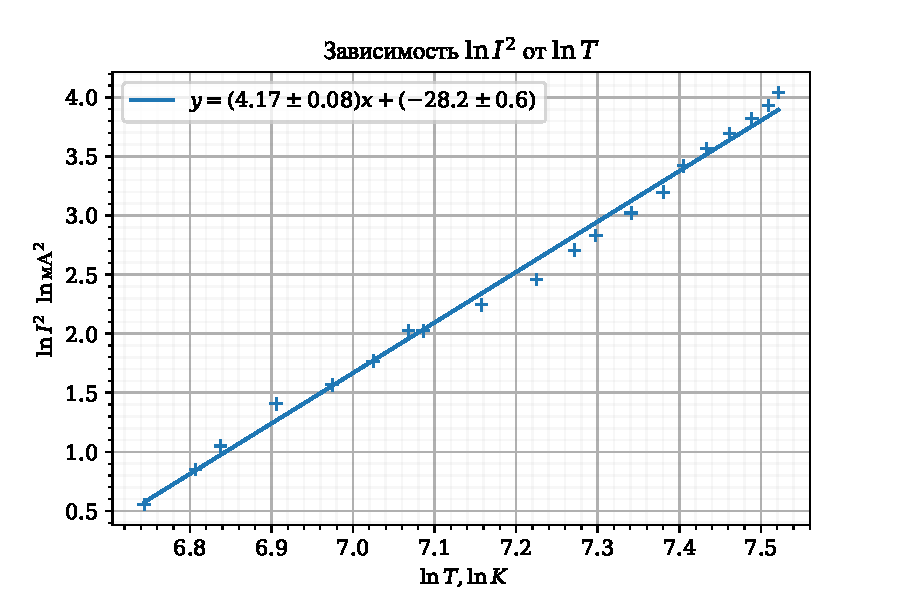
\includegraphics[scale=1]{plot_8_1.pdf} 
\label{plot}
\caption{График зависимости силы тока от температуры в логарифмических координатах}
\end{figure}
\item \textbf{Определения постоянных Планка и Стефана-Больцмана}
\begin{enumerate}
\item Из формулы (2) получим, что постоянная Стефана-Больцмана выражается как:
\begin{equation}
\sigma = \frac{W}{\varepsilon_TST^4}
\end{equation}
где $\varepsilon_T$ -- табличное значение коэффициента излучения при различных температурах\\
$S$ -- эффективная площадь излучающей поверхности, $S = 0.36$ см\\
T -- температура нити\\
W -- мощность\\
$\sigma$ -- постоянная Стефана-Больцмана\\\\
Погрешность в данном случае можно выразить как 
\[\Delta\sigma = \sqrt{\left(\frac{\Delta W}{W}\right)^2 + 4\left(\frac{\Delta T}{T}\right)^2}\]
При расчетах берем среднее сопротивление, равное $R = 0.14 $ Ом, предполагая линейную зависимость между силой тока и сопротивлением при данном диапазоне температур
\item Полученные данные для постоянной Стефана-Больцмана занесем в таблицу 3
\begin{table}[h!]
\centering
\begin{tabular}{|l|l|l|l|l|l|l|l|l|l|}
\hline
T, K                          & 1750 & 1815 & 1877 & 1917 & 1964 & 2013 & 2061 & 2098 & 2120 \\ \hline
$\sigma$, СГС $10^{-5}$       & 5.16 & 5.03 & 4.72 & 4.72 & 4.37 & 4.31 & 4.32 & 4.27 & 4.05 \\ \hline
$\Delta\sigma,$ СГС $10^{-5}$ & 0.08 & 0.08 & 0.07 & 0.07 & 0.07 & 0.06 & 0.06 & 0.06 & 0.06 \\ \hline
\end{tabular}
\caption{Значения постоянной Стефана-Больцмана}
\label{SB}
\end{table}

\item По полученным данным получим среднее значение константы Стефана-Больцмана:
\[\overline{\sigma} = (4.55 \pm 0.08)\cdot 10^{-5} \frac{\text{эрг}}{\text{см}^2K^4c}\]
\item Определим постоянную Планка по формуле: 
\[h = \sqrt{\frac{2\pi^2k_{\text{Б}}^4}{15c^2\sigma}}\]
Подставляя усредненное значение $\sigma = \overline{\sigma}$ получим $h = (7.1 \pm 0.2)\cdot 10^{-27}$ эрг$\cdot$с
\end{enumerate}
\item \textbf{Измерение яркостной температуры неоновой лампочки}\\
Подключим неоновую лампочку к источнику питания и направим на нее пирометр. Значение на пирометре соответствует температуре $T = 900 ^oC$, но при касании лампочка является холодной.\\
Явление связано с тем, что излучение лампочки происходит в дискретном спектре, в отличии от разогретых тел
\end{enumerate}
\paragraph{Выводы:}
\begin{enumerate}
\item На модели АЧТ убедились в исправности пирометра
\item Убедились, что при одной и той же термодинамической температуре может быть разной яркостная температура у различных материалов
\item Проверили закон Стефана-Больцмана ($W \sim T^4$)
\item Нашли значение постоянной Стефана-Больцмана, равной $\sigma = (4.55\pm 0.08)\cdot 10^{-5} \frac{\text{эрг}}{\text{см}^2K^4c}$
\item Нашли значение постоянной Планка $h = (7.1 \pm 0.2)\cdot 10^{-27}$ эрг$\cdot$с
\item Убедились в том, что термодинамическая температура для неоновой лампочки гораздо ниже яркостной. Объясняется тем, что излучение лампочки происходит в дискретном спектре
\end{enumerate}
\end{document}